\documentclass[10pt, a4paper, twoside]{article}

% Set up the standard margins for the document
% 42.2 left & 15.5 right is same as Forsling, Neymark
% 21.3 top  & 20 bottom is same as Olofsson
\usepackage[left=25.5mm, right=25.5mm, top=21.3mm, bottom=20mm]{geometry}

% Input file character encoding (kinda useless if we don't
% use åäö and stuff, but it doesn't hurt to have it)
\usepackage[utf8]{inputenc}
%\usepackage[swedish]{babel}
\usepackage{caption}
\usepackage{subcaption}
% Block Comments
\usepackage{comment}

% No indentation in new paragraph
\usepackage{parskip}

% To include graphics
\usepackage{graphicx}

% More mathematical symbols and fonts
\usepackage{amsmath}
\usepackage{amsfonts}
\usepackage{amssymb}

% Simple list
\usepackage[ampersand]{easylist}
\ListProperties(Hide=100, Hang=true, Progressive=5ex, Style*=$\bullet$ ,
Style2*=-- ,Style3*=$\circ$ ,Style4*=\tiny$\blacksquare$ )


% Clickable internal links
\usepackage{hyperref}
\usepackage[all]{hypcap} % without this the link takes you to the caption, not the top of the image
\hypersetup{ % Settings for links in documnet
	setpagesize = false, % Don't allow hyperref to change page size. Tips från Micke Olofsson
	colorlinks = true,   % No boxes around links
	linkcolor = black,citecolor = black,filecolor = black,urlcolor = black, % don't color links
}

% To include to first page pdf file
\usepackage{pdfpages}

% Add section number to equation and figure number (ex: 5.11 instead of simply 11)
\numberwithin{equation}{subsection}
\numberwithin{figure}{section}
\numberwithin{table}{section}

% Show program code listings in document
\usepackage{listings}

%
% Header stuff
%
\usepackage{fancyhdr}
\setlength{\headheight}{15pt}

\fancyhf{}
\fancyhead[LE, RO]{\thepage}
\fancyhead[RE]{TSBB11 2013: Specification of Requirements}
\fancyhead[LO]{Kitchen Occupation}

\fancypagestyle{plain}{ %
\fancyhf{} % remove everything
\renewcommand{\headrulewidth}{0pt} % remove lines as well
\renewcommand{\footrulewidth}{0pt}}
%
% End header stuff
%

%
% Definitions of commands for the requirement table
%

\newcounter{reqCounter}[section]
\newcommand{\reqnum}
{
	\addtocounter{reqCounter}{1}
	\textbf{\arabic{section}.\arabic{reqCounter}}
}

\newcommand{\reqtable}[1]
{
	\vspace{0.5cm}
	\begin{center}
	\begin{Large}
	\begin{tabular}{|c|p{12.5cm}|c|}
		\hline
		\large{\textbf{Req.}} & \large{\textbf{Description}} & \large{\textbf{Type}} \\
		\hline
	#1
	\end{tabular}
	\end{Large}
	\end{center}
}

\newcommand{\addreq}[2]
{
	\large{\reqnum} & \normalsize{#1} & \large{\textbf{#2}} \\
	\hline
}

\begin{document}

% First page

\includepdf{Cover/cover.pdf}


% Project identity page
\newpage
\pagestyle{fancy}
\pagenumbering{roman}
\setcounter{page}{2} % sets the current page number to 2 

% Group info
\begin{center}
    \vspace*{4\baselineskip}

	\textbf{\huge Project Kitchen Occupation} \\
	\vspace*{0.5\baselineskip}
	Bilder och Grafik CDIO, HT 2013 \\
	Department of Electrical Engineering (ISY), Link\"{o}ping University
	
	\vspace*{2\baselineskip}
	\textbf{\LARGE Participants}


	{\footnotesize 
	\begin{tabular}{|p{2.7cm}|p{1cm}|p{5cm}|p{2cm}|p{3.4cm}|}
		\hline
		\textbf{Name} & \textbf{Tag} & \textbf{Responsibilities} & \textbf{Phone} & \textbf{E-mail} \\
		\hline
		Mattias Tiger & MT & Project manager & 073--695\,71\,53 & matti166@student.liu.se \\
		\hline
		Erik Fall & EF & -- & 076--186\,98\,84 & erifa226@student.liu.se \\
		\hline
		Gustav Häger & GH & System integration & 070--649\,03\,97 & gusha124@student.liu.se \\
		\hline
		Malin Rudin & MR & -- & 073--800\,35\,77 & malru103@student.liu.se \\
		\hline
		Alexander Sjöholm & AS & -- & 076--225\,11\,74 & alesj050@student.liu.se \\
		\hline
		Martin Svensson & MS & Documentation & 070--289\,01\,49 & marsv106@student.liu.se \\
		\hline
		Nikolaus West & NW & Testing & 073--698\,92\,60 & nikwe491@student.liu.se \\
		\hline
	\end{tabular}
	}

{\footnotesize 
\vspace{0.5\baselineskip}
\textbf{Homepage}: TBA \\
\vspace{1\baselineskip}

\textbf{Customer}: Joakim Nejdeby, Link\"{o}ping University, Origo 3154 \\
\textbf{Customer contact}: 013--28\,17\,57, joakim.nejdeby@liu.se \\
\textbf{Project supervisor}: Fahad Khan, Link\"{o}ping University, fahad.khan@liu.se \\
\textbf{Examiner}: Michael Felsberg, michael.felsberg@liu.se \\
}

\end{center}


% table of contents
\newpage
\tableofcontents
\listoffigures
%\listoftables


% Document history page
\newpage
\vspace*{5\baselineskip}

\begin{center}
\textbf{\LARGE Document history}

{ \footnotesize 
\begin{tabular}{|p{1cm}|p{2.0cm}|p{6.5cm}|p{2cm}|}
	\hline
	\textbf{Version} & \textbf{Date} & \textbf{Changes} & \textbf{Sign} \\
	
	\hline
	0.1 & 2013--09--09 & Initial draft & MS \\
	\hline
	0.2 & 2013--09--18 & Scrum adaptation & MT \\
	\hline
	1.0 & 2013--09--24 & Final Document & All \\
	\hline
	1.1 & 2013--11--27 & Revision of several requirements due to changed conditions combined with the realization that depth information is needed to reach good enough performance. & MS, EF, MT \\
	
	\hline
	 &  &  &   \\
	
	\hline
\end{tabular}
}
\end{center}


% Blank page
%\newpage
%\thispagestyle{empty}
%\mbox{}

%
% Content start
%
\newpage
\pagenumbering{arabic}


\newpage
\section{Introduction}
\label{sec:introduction}
What to write here? maybe nothing.

\subsection{About this document}
This docment, is the user manueal....


\newpage
\section{System Overview}
\label{sec:system_overview}
Below is an overview of the entire system. Data collection from several rooms are performed simultaneously, and processed data is presented to the user through a web page.

\vspace{0.5cm}
\begin{figure}[htb]
	\centering
	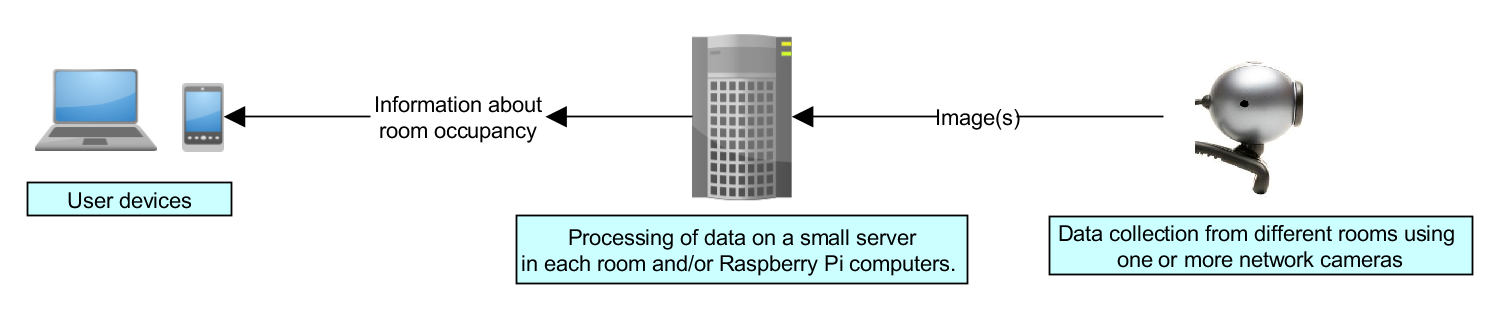
\includegraphics[width=170mm]{images/system_overview.png}
	\caption[System overview]{\textit{A simplified overview of the system}}
	\label{fig:block_overview2_fig}  %Skapar referens till figuren
\end{figure}

\subsection{Rough description of the system}
The camera(s) used to collect data are connected to a local network via Ethernet cables. The main program collects data from the cameras in a room to perform an estimation of room usage intensity, which is then presented to the user in an understandable format, e.g. estimated waiting time.

\subsection{Components}
The main components of the system is of course the cameras, as well as the software running on the central server.

\subsubsection{Hardware}
The cameras are network cameras powered via Ethernet cable, mounted in way that allows for good performance and low installation costs. The hardware is described more thoroughly on this in section \ref{sec:hardware}.

\subsubsection{Software}
The software will be running on a central server, where both image processing and estimation of queue size and waiting time takes place. For a more thorough description of the image processing and estimation programs, see section \ref{sec:software}.

\subsection{Usability and installation}
In order to create a system that is cheap to use and install, it needs to be easy to set up, which is why a user's manual and an installation/calibration program is provided with the system if necessary. As for the usability, relevant data is presented to the user on a web page (see section \ref{sec:usage}). 



\newpage
\section{Hardware}
\label{sec:hardware}

Since the system is to be able to run on two different platforms, the hardware requirements differ a lot depending on which system being considered. In the case of Raspberry Pi computers being used, all cameras each have their own Raspberry Pi processing unit where image processing takes place. In case of a central image processing unit (laptop, server or desktop computer), image processing from all cameras in the room take place on this central unit.


\begin{figure}[htb]
	\centering
	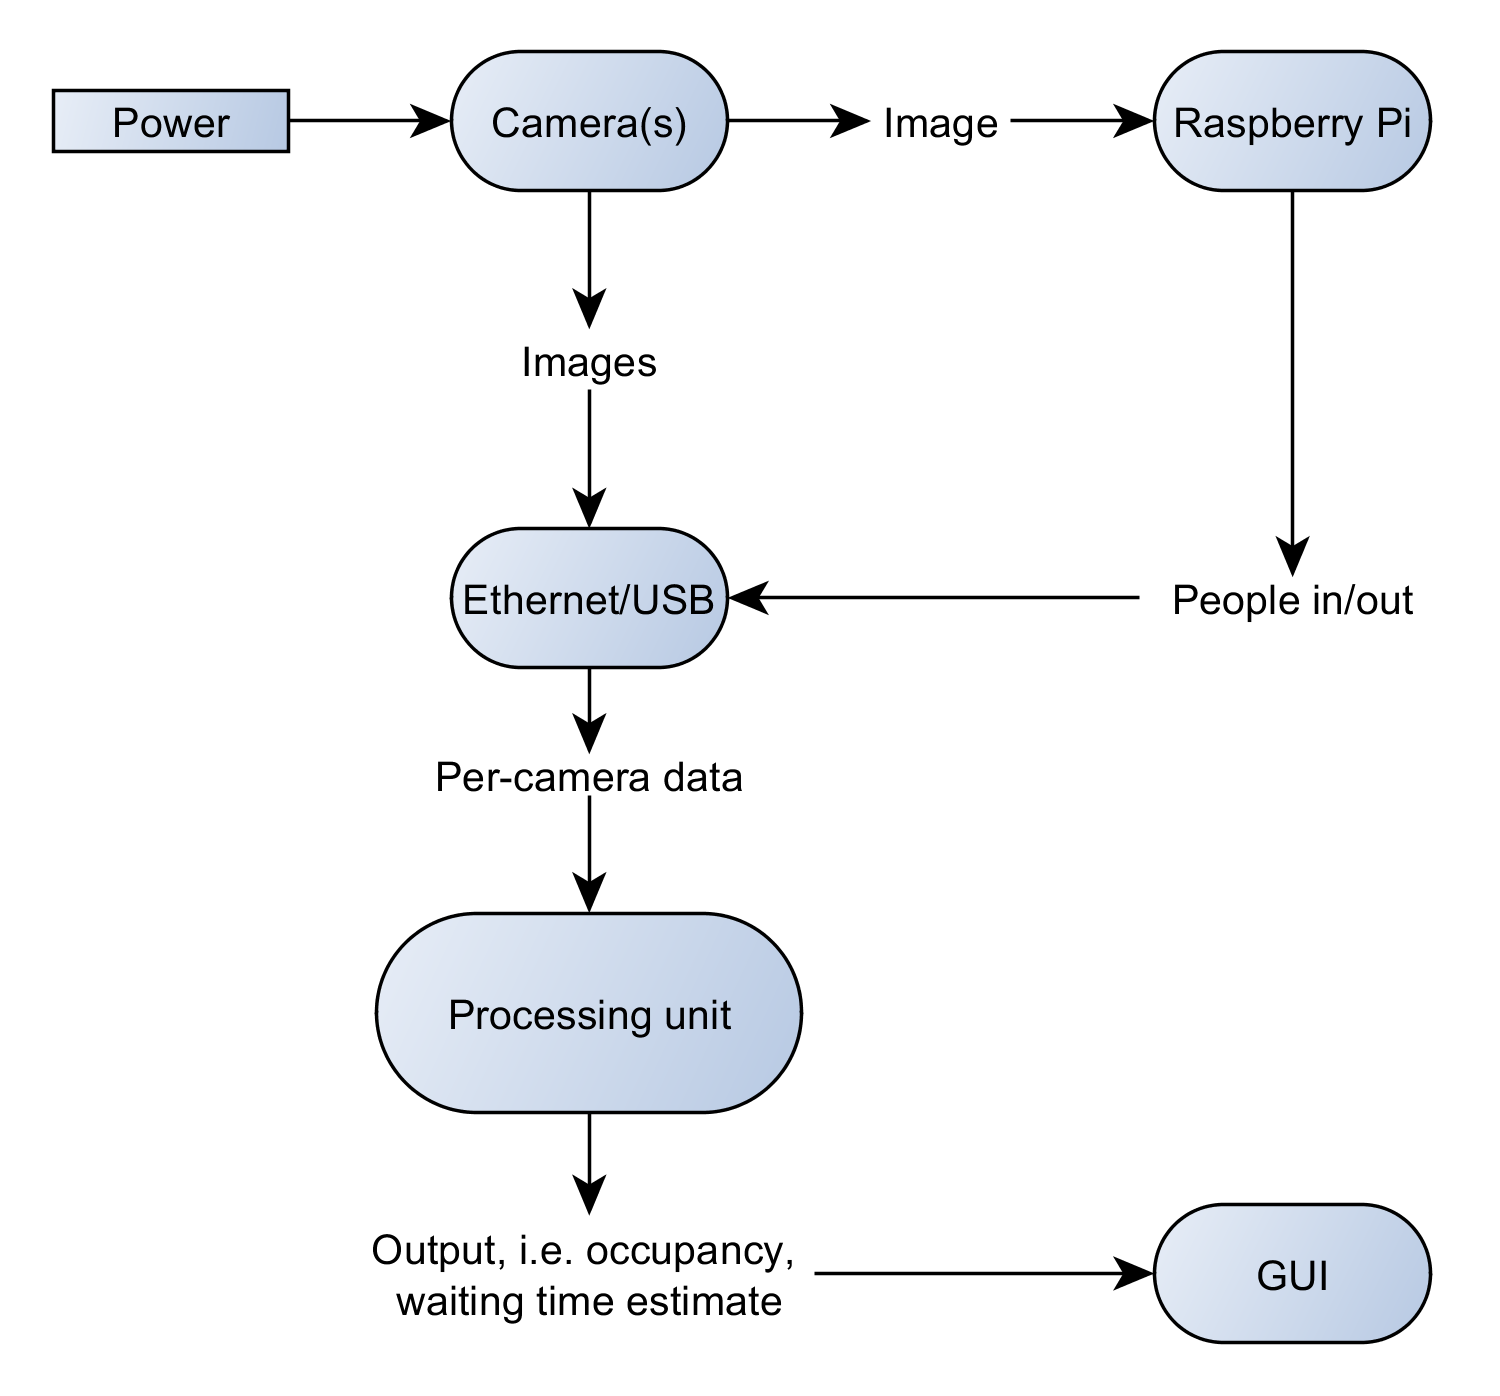
\includegraphics[width=160mm]{images/Hardware.png}
	\caption{\textit{Flowchart displaying data flow between hardware modules}}
	\label{fig:block_overview_fig}  %Skapar referens till figuren
\end{figure}
\newpage

\subsection{Limitations}
The hardware is limited by budget, Internet connection and the source of power. The cost is limited to approximately 15.000 SEK per room, including installation costs. The budget limits performance of the cameras e.g. resolution and number of cameras. The connection from the cameras to the processing unit(s) needs to be stable and have a bandwidth good enough for sending live video from the cameras. Additionally, no image data may be transmitted over public networks.   
\newpage
\subsection{Hardware Requirements}
\label{sec:hardware_req}
\reqtable
{
	\addreq{The system uses network cameras powered via Ethernet.\newline \textbf{Revised 2013-11-27:} The system uses cameras connected to a laptop (or similar mid-end processing device) via network or USB.}{1}	
	\addreq{The system can operate using high resolution ($>$2 Mpixel) cameras}{1}
	\addreq{Lower resolution cameras can be used}{2}
	\addreq{The application can run using the processing power provided by the costumer.\newline \textbf{Canceled 2013-11-27: }No processing power will be provided by the customer within the delivery time.}{--}
	\addreq{The application can run using a mid-end processing device (e.g. a laptop or desktop computer).\newline \textbf{Revised priority 2013-11-27:} The cancellation of previous req.(\textbf{3.4}) causes priority to change \textbf{from 2 to 1.}}{1}
	\addreq{The application can run using a low-end processing device.\newline	\textbf{Revised priority 2013-11-27:} Revised due to a request from customer that the system is able to run on a Raspberry Pi. Priority changed \textbf{from 3 to 2.}}{2}
}

\newpage
\section{Software}
\label{sec:software}
The software part of the system performs all the image processing and analysis needed to detect usage of a room. It will also be cablable of predicting future room occupancy degree based on historical usage. 

A website for the project will be published using the wordpress CMS or using GitHubs webpage services, it will describe the project and its participants.
 
\subsection{External dependencies}
The software is written using the OpenCV library to handle the image processing, and when possible interfacing with cameras. 
Any visualization and debugging tools are written using the Qt framework. 
OpenNI is used for accessing the Kinect camera. 
An HTTP library is used to handle communication with LiUs REST API.
Cmake and any C++11 capable compiler can be used to compile the source code to binary.

The website will be hosted on a standard LAMP stack.

\subsection{Compatibility}
The software is possible to build for most major platforms (Windows/OS X). A REST API is used to communicate the results.

\subsection{Limitations}
For integrity reasons no personally identifiable information can be stored or reported by the system. The processing is done locally for each camera on a Raspberry PI or on a remote computer connected via network or USB. Depending on which of these hardware configurations is used, the computational power will differ and therefore limiting or enabling the use of computational-heavy algorithms.  

\subsection{Software Requirements}
\label{sec:software_req}
\reqtable
{	
	\addreq{The system runs on Windows based plattforms}{1}
	\addreq{The system runs on OS X}{1}
	\addreq{\textbf{Added 2013-11-27:} The system runs on Raspberry PI}{2}
	\addreq{The system is modular with respect to the camera manufacturer and/or network API.\newline
			\textbf{Revised 2013-11-27:} The system is modular with respect to any OpenCV-compatible camera and network API}{1}
	\addreq{The system must not store image data}{1}
}

\newpage
\section{Performance}
\label{sec:performance}
The performance of the system refers to what problems the system solves and the degree to which it solves them. The problem that the system solves is giving indications to how long the wait will be for use of microwaves in the student kitchen. The simplest indicator for this is simply the amount of people in the kitchens. This is made slightly more complicated by the potential presence of more than one door into the room. The amount of people in the room is also easily verified by hand, meaning that performance with regard to this indicator is easily defined and quantified. Other indicators of the length of waiting are detection of a queue, rough classification of the severity of the queue, and a directly estimated waiting time. The system performance on these indicators are all increasingly both hard to define and measure. The inclusion of methods to evaluate and test these more difficult indicators are therefore necessary.

\subsection{Reliability}
The system should ideally be able to perform reliably under varying lighting conditions, while also being able to handle people with varying hair color and whearing a large varaiaty of different clothes, jackets, hats. It is preferable that the system also handles bags, trolleys etc. without counting them as extra people. 

\subsection{Quality control}
The system is thoroughly tested throughout development to ensure high quality. The core computer vision functionality is also continuously tested against a test data set that is never used to train or tune any algorithms. 
\newpage

\subsection{Performance requirements}
The performance requirements listed below assume that it is possible to have cameras placed over each door. Removing this assumption results in increasing the type number by one (e.g. from 1 to 2).   
\label{sec:performance_req}
\reqtable
{
	\addreq{The system is able to count the number of people entering and leaving the room, where the room has one door.}{1}
	\addreq{The system is able to count the number of people entering and leaving the room, where the room has two doors.}{1}
	\addreq{The system keeps track of the amount of people in the room at any one time, given that it can count the number of people passing through each door.}{1}
	\addreq{The system knows if there is a queue to enter the room.\newline
			\textbf{Canceled 2013-11-27:} Redundant because of next requirement in the table.}{1}
	\addreq{A rough classification of the queue size/severity is presented by the system, where the room has one door.}{1}
	\addreq{A rough classification of the queue size/severity is presented by the system, where the room has two or more doors.}{2}
	\addreq{The system gives a model based estimate of the waiting time that is more informative than the rough queue classifications. }{2}
	\addreq{The system can handle daily variations in lighting conditions such that other performance metrics are not affected.\newline \textbf{Clarified 2013-11-27:} The system can handle daily indoor lightning conditions such that other performance metrics are not widely affected. }{1}
	\addreq{The system handles sudden changes in lighting (e.g. a blackout) without crashing and keeping track of potentially induced knowledge gaps.}{2}
	\addreq{The system is tested against a data set that covers a wide variety of the most common cases.\newline 
			\textbf{Revised 2013-11-27:} The system is tested against a data set that covers the most common cases.}{1}
}

\newpage
\section{Usage and Installation}
\label{sec:usage}
This section describes what is required by the system in terms of usage and installation. It also covers what is wanted by the user. 

\subsection{Installation}
The installation consists of the placement of one or more cameras, connection of these via Ethernet to a computer, and installation of the software on that computer. The cameras should be placed as described in the user manual with focus on vision rather than precise positioning. The connection via Ethernet is completely provided by the user.     

Once installed the system needs a calibration which is preformed by the user in the calibration program.

The installation and calibration process is described in detail to the user in the user manual.

\subsection{Usage}
When the system is properly installed it can be maneuvered by the user through the interface. The user can now start adding cameras together from the interface. Now the system will start keeping track of the room and continuously provide the user with occupancy statistics about the room. 

\subsection{Maintenance}
The system should be able to run continuously once started, without further maintenance. Additional cameras can not necessarily be added on the fly. 

\subsection{Continued development}
The user interface is initially not prioritized as this is a project mainly in computer vision. This will leave some GUI features open for future development. 

\subsection{Operational requirements}
The user is assumed to have some minor computer skills, but no knowledge whatsoever about computer vision. 


\label{sec:ui_req}
\reqtable
{
	\addreq{The installation proces requires a short manual and no knowledge about advanced computer vision}{1}
	\addreq{Calibration of the system is performed via a calibration program}{1}
	\addreq{The system is self-calibrating}{2}
	\addreq{Software for adding new cameras and/or rooms is provided with the system. \newline
			\textbf{Revised 2013-11-27:} Only single-room - many sensors support is provided.}{1}
	\addreq{Results are presented on the project group webpage}{1}
	\addreq{System is avaliable as an App on AppStore/Android Market}{3}
}

\newpage
\section{Documentation}
\label{sec:documentation}
The following documents are produced along the course of the project.

\subsection{Project plan}
The outline of the project is described in the project plan. It specifies the nature of the project, responsibilities, resources available, the organization of the project and development methods. It also contains the preliminary Product backlog with preliminary priorities and estimated finish dates based on the priorities.

\subsection{User's manual}
To help the user to install and use the product, a user's manual is presented. It is a description of the installation and usage of the product.

\subsection{Scrum review document}
After each sprint a Scrum review document is produced containing the sprint backlog together with the result of the sprint and a review.

\subsection{Technical report}
At the end of the project the result of the project is documented in a technical report. This report is a detail description of the different aspects of the project, such as hardware and software solutions, limitations of the system and further developments.

\subsection{Documentation Requirements}
\label{sec:documentation_req}
\reqtable
{
	\addreq{A project plan providing an outline of responsibilities and development methods has to be presented to the supervisor}{1}
	\addreq{At the end of the project a technical report is delivered to the customer and course examiner}{1}
	\addreq{A user's manual will be delivered with the technical report}{1} 
	
}


\newpage
\section{Delivery}
\label{sec:delivery}
A partial system will be delivered at the Mid-term checkpoint and the full system along with documentation is delivered at the final delivery deadline.

\subsection{Mid-term checkpoint}
A partially working system is delivered (What this means will be clarified here once the project plan is finalized).

\subsection{Final delivery}
A kitchen occupancy software system, fullfilling atleast all requirements of type 1, is delivered to the customer.
Full documentation specified in section \ref{sec:documentation} is delivered to the customer.
A project web page is online with a short introduction to the project and a video demonstration of the system.

\subsection{Delivery dates}
\label{sec:delivery_req}
\begin{center}
	\begin{Large}
	\begin{tabular}{|p{10.5cm}|c|}
		\hline
		\large{This document} & \large{\textbf{2013-09-24}} \\
		\hline
		\large{Project plan} & \large{\textbf{2013-09-24}} \\
		\hline
		\large{Sprint review document} & \large{\textbf{At the end of each sprint}} \\
		\hline
		\large{Final product} & \large{\textbf{2013-12-13}} \\
		\hline
		\large{Technical report} & \large{\textbf{2013-12-13}} \\
		\hline
		\large{User's manual} & \large{\textbf{2013-12-13}} \\
		\hline
		\large{Final presentation} & \large{\textbf{2013-12-19}} \\
		\hline	
		
	\end{tabular}
	\end{Large}
\end{center}


%
% Bibliography
%

% Force a blank page so the bibliography starts on a new page.
% Comment out if not necessary
%\newpage

%\thispagestyle{fancy}
%\mbox{}
%\newpage
%\begin{thebibliography}{9}
\addcontentsline{toc}{section}{References} % Add an entry for this in the table of contents

\bibitem{Gardel}
	Gardel, A., Bravo, I., Jimenez, P., Lazaro, J.L. \& Torquemada, A.\\
	``\textit{Statistical Background Models with Shadow Detection for Video Based Tracking},''\\ Intelligent Signal Processing, 2007. WISP 2007. IEEE International Symposium on?? Page: 1-6.
	
\bibitem{Zivkovic}
	Zivkovic, Z. \& Heijden, F.\\
	``\textit{Efficient Adaptive Density Estimation per Image Pixel for the Task of Background Subtraction},''\\
	Pattern recognition letters, Vol. 27, No. 7. (2006), pp. 773-780.

\vspace{2cm}
\LARGE{\textbf{EXAMPLE REFERENCES ONLY, REMOVE BEFORE HANDING IN}}
\normalsize
\bibitem{CVBook}
	Sonka, M., Hlavac, V. \& Boyle, R. 
	\emph{Image Processing, Analysis, and Machine Vision}.\\
	Toronto: Thompson Learning,
	cop. 2008, 3rd ed.,
	ISBN 0495244384.
	
\bibitem{Wood}
	Wood, J. (2007)
	``\textit{Statistical Background Models with Shadow Detection for Video Based Tracking},''\\
	Master thesis, Linköping University, Department of Electrical Engineering.	

\bibitem{DSPBook}
	Gustafsson, F., Ljung, L. \& Millnert, M.
	\emph{Signal Processing}.\\
	Studentlitteratur, Lund, Sweden,
	2011, 1st ed.,
	ISBN 978--91--44--05835--1.

\bibitem{MOTA}
	Bernardin, K. \& Stiefelhagen, R (2008)\\
	``\textit{Evaluating Multiple Object Tracking Performance: The CLEAR MOT Metrics},''\\
	Interactive Systems Lab, Institut für Theoretische Informatik,\\
	Universität Karlsruhe, 76131 Karlsruhe, Germany

\bibitem{CAVIAR}
	``\textit{CAVIAR: Context Aware Vision using Image-based Active Recognition},''\\
	EC Funded CAVIAR project/IST 2001 37540\\
	http://homepages.inf.ed.ac.uk/rbf/CAVIAR/
	

%\bibitem{somePaper}
%	Q. Lastname,
%	``Some article title,''
%	\emph{Some scientific journal},
%	vol.~1337, no.~1337,
%	pp.~666--1337,
%	month.~1337.

\end{thebibliography}



\end{document}
